% !TeX root = main.tex

% 双语图题：沿用 main.tex 已加载的 caption 和 ctex。

\newcommand{\methodbicaption}[3]{%
  \begingroup
  \captionsetup{font=methodfive,labelfont=bf,textfont=bf,
    labelformat=methodfiglabel,labelsep=quad,
    justification=centering,singlelinecheck=false}%
  \captionof{figure}[#1]{#1\protect\\%
    \textbf{Figure~\thefigure\quad #2}}%
  \label{#3}%
  \endgroup
}

\section{语义分割模型（BiMSeg）的构建与应用}
\label{sec:method}

% 仅调整方法部分的标题间距；作用域到文件末尾。
\begingroup
\ctexset{
  subsection = {beforeskip = 12pt, afterskip = 8pt},
  subsubsection = {beforeskip = 12pt, afterskip = 8pt}
}

\subsection{BiMSeg 双向多尺度网络语义分割算法}

\subsubsection{BiMSeg 整体网络架构}
\begingroup
  \centering
  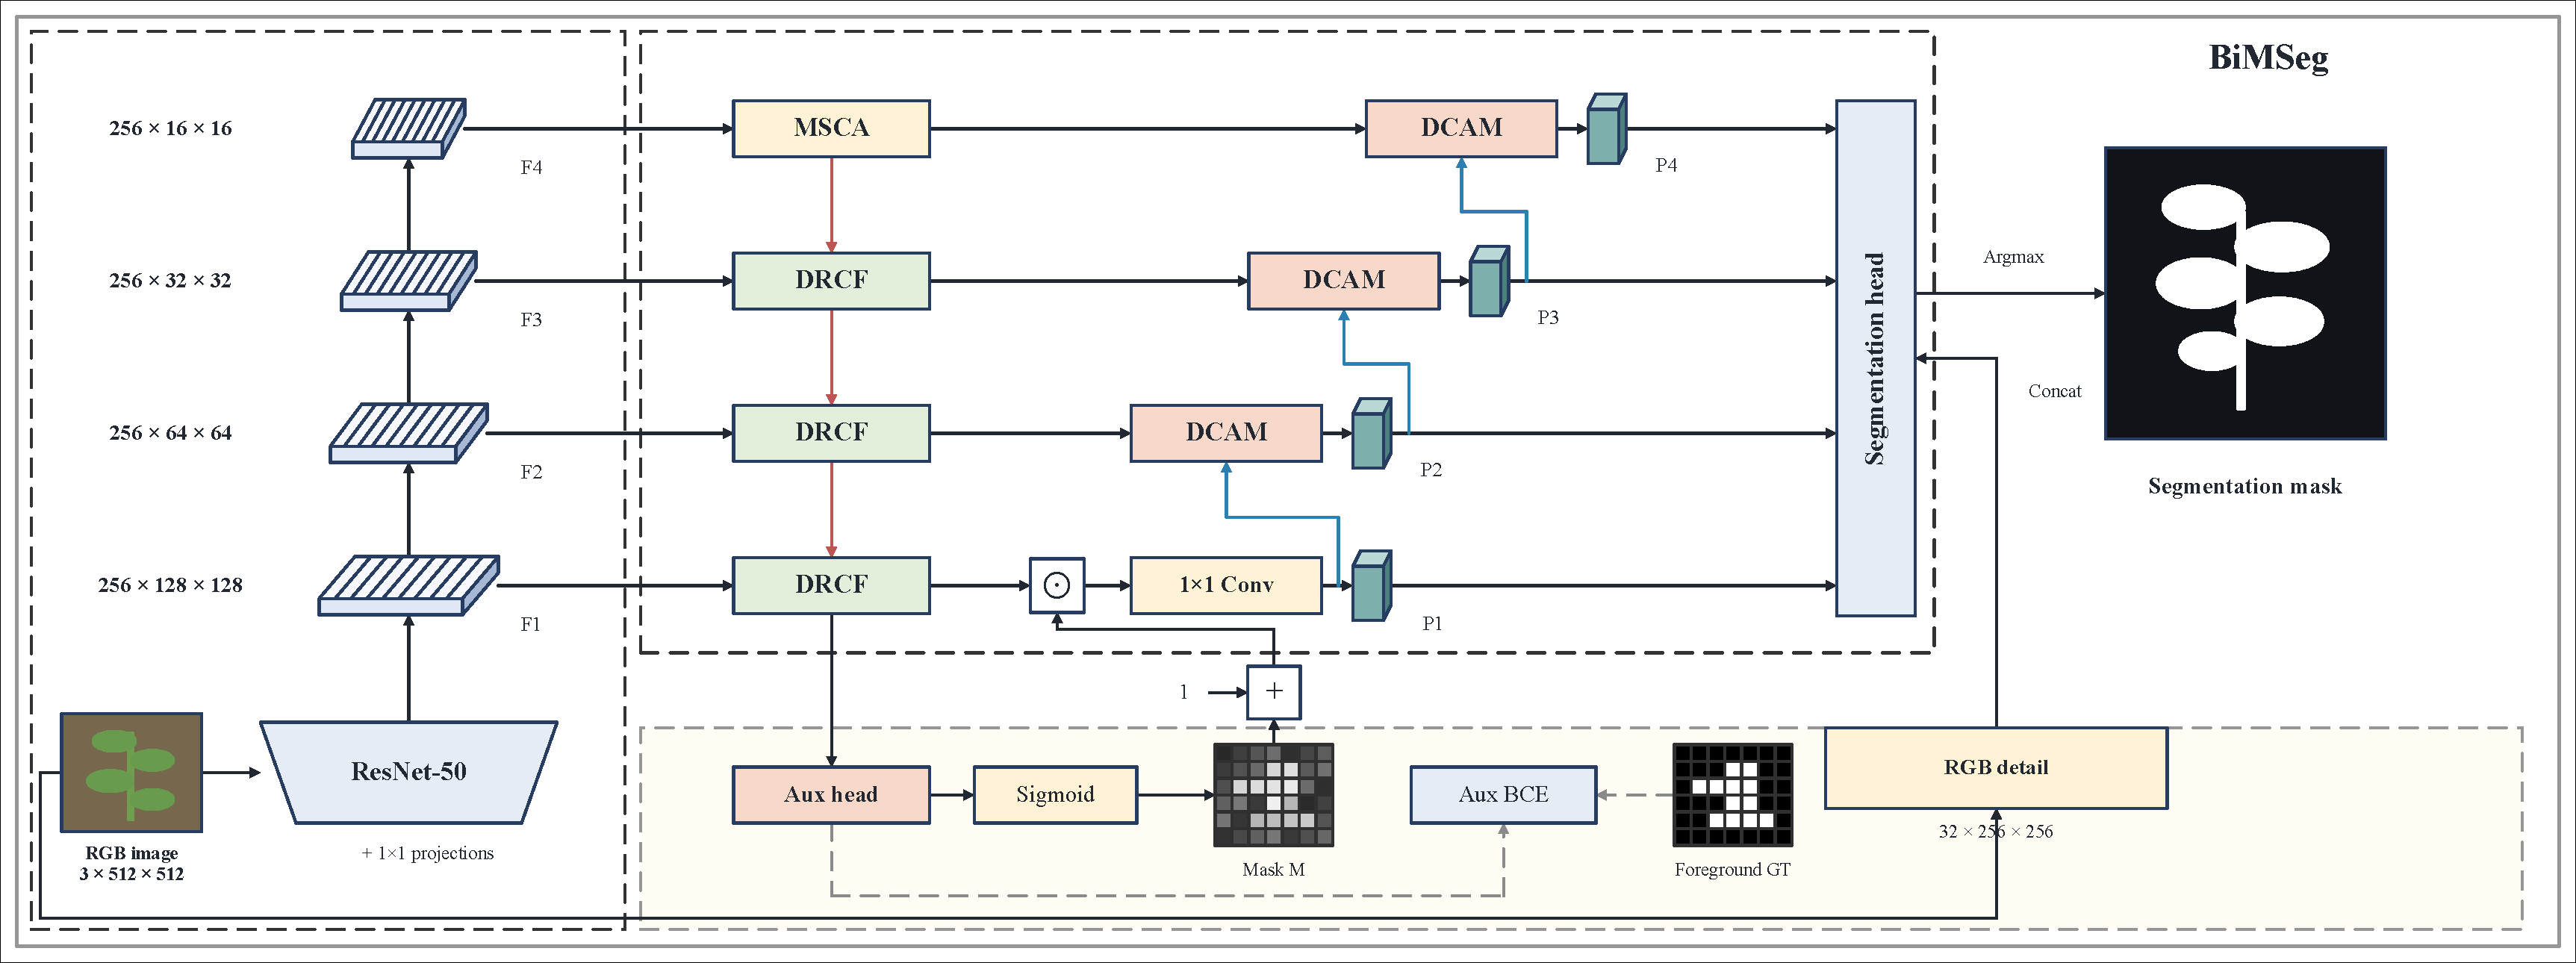
\includegraphics[width=\linewidth]{BiMSeg_Architecture_Polished.pdf}\par
  \begin{spacing}{1}
    \methodbicaption{BiMSeg 整体网络架构}
      {Overall architecture of BiMSeg}{fig:architecture}
  \end{spacing}
  \par
\endgroup
\addvspace{6pt}

针对禾本科植物图像中目标尺度变化、叶片相互遮挡及细长结构
难以完整分割的问题，本文提出双向多尺度分割网络
（Bidirectional Multi-scale Segmentation Network，BiMSeg）。
网络由 ResNet50 编码器、多尺度稀疏交叉注意力模块
（Multi-scale Sparse Cross-Attention，MSCA）、
动态关系与上下文融合模块
（Dynamic Relation and Context Fusion，DRCF）、
差异引导的跨尺度自适应调制模块
（Discrepancy-guided Cross-scale Adaptive Modulation，DCAM）
及分割预测头组成。
通过自顶向下的语义传递与自底向上的细节反馈，
实现深层语义、浅层结构及图像细节的协同整合。

如图~\ref{fig:architecture} 所示，
给定输入图像 \(I\in\mathbb{R}^{3\times H\times W}\)，
采用 ResNet50 编码器\papercite{he2016resnet}
提取四个层级的特征，
并通过 \(1\times1\) 卷积将通道数统一为 \(C=256\)，
得到特征集合 \(\{F_1,F_2,F_3,F_4\}\)。
其空间分辨率依次为输入的
\(1/4\)、\(1/8\)、\(1/16\) 和 \(1/32\)。
最深层特征 \(F_4\) 经 MSCA
聚合多尺度局部信息与空间上下文，
得到增强特征 \(F_4'\)，
并令 \(G_4=F_4'\)。
随后，三级 DRCF 分别融合
\(G_4\) 与 \(F_3\)、\(G_3\) 与 \(F_2\)、
\(G_2\) 与 \(F_1\)，
依次生成 \(G_3\)、\(G_2\) 和 \(G_1\)，
完成自顶向下的语义传递。
为简化表示，后续特征尺寸描述中省略批量维度。

基于最浅层融合特征 \(G_1\)，
辅助预测头生成前景概率图 \(M\)，
通过残差加权增强前景响应，
并经通道映射得到 \(P_1\)。
自底向上路径以 \(P_1\) 为起点，
利用三级 DCAM 分别与 \(G_2\)、\(G_3\) 和 \(G_4\)
交互，依次生成 \(P_2\)、\(P_3\) 和 \(P_4\)，
将浅层细节逐级反馈至深层表征。
最后，对齐并融合四个层级的输出，
结合 RGB 细节分支生成与输入图像等分辨率的类别响应，
得到最终分割结果。

\subsubsection{多尺度稀疏交叉注意力模块（MSCA）}
\begingroup
  \centering
  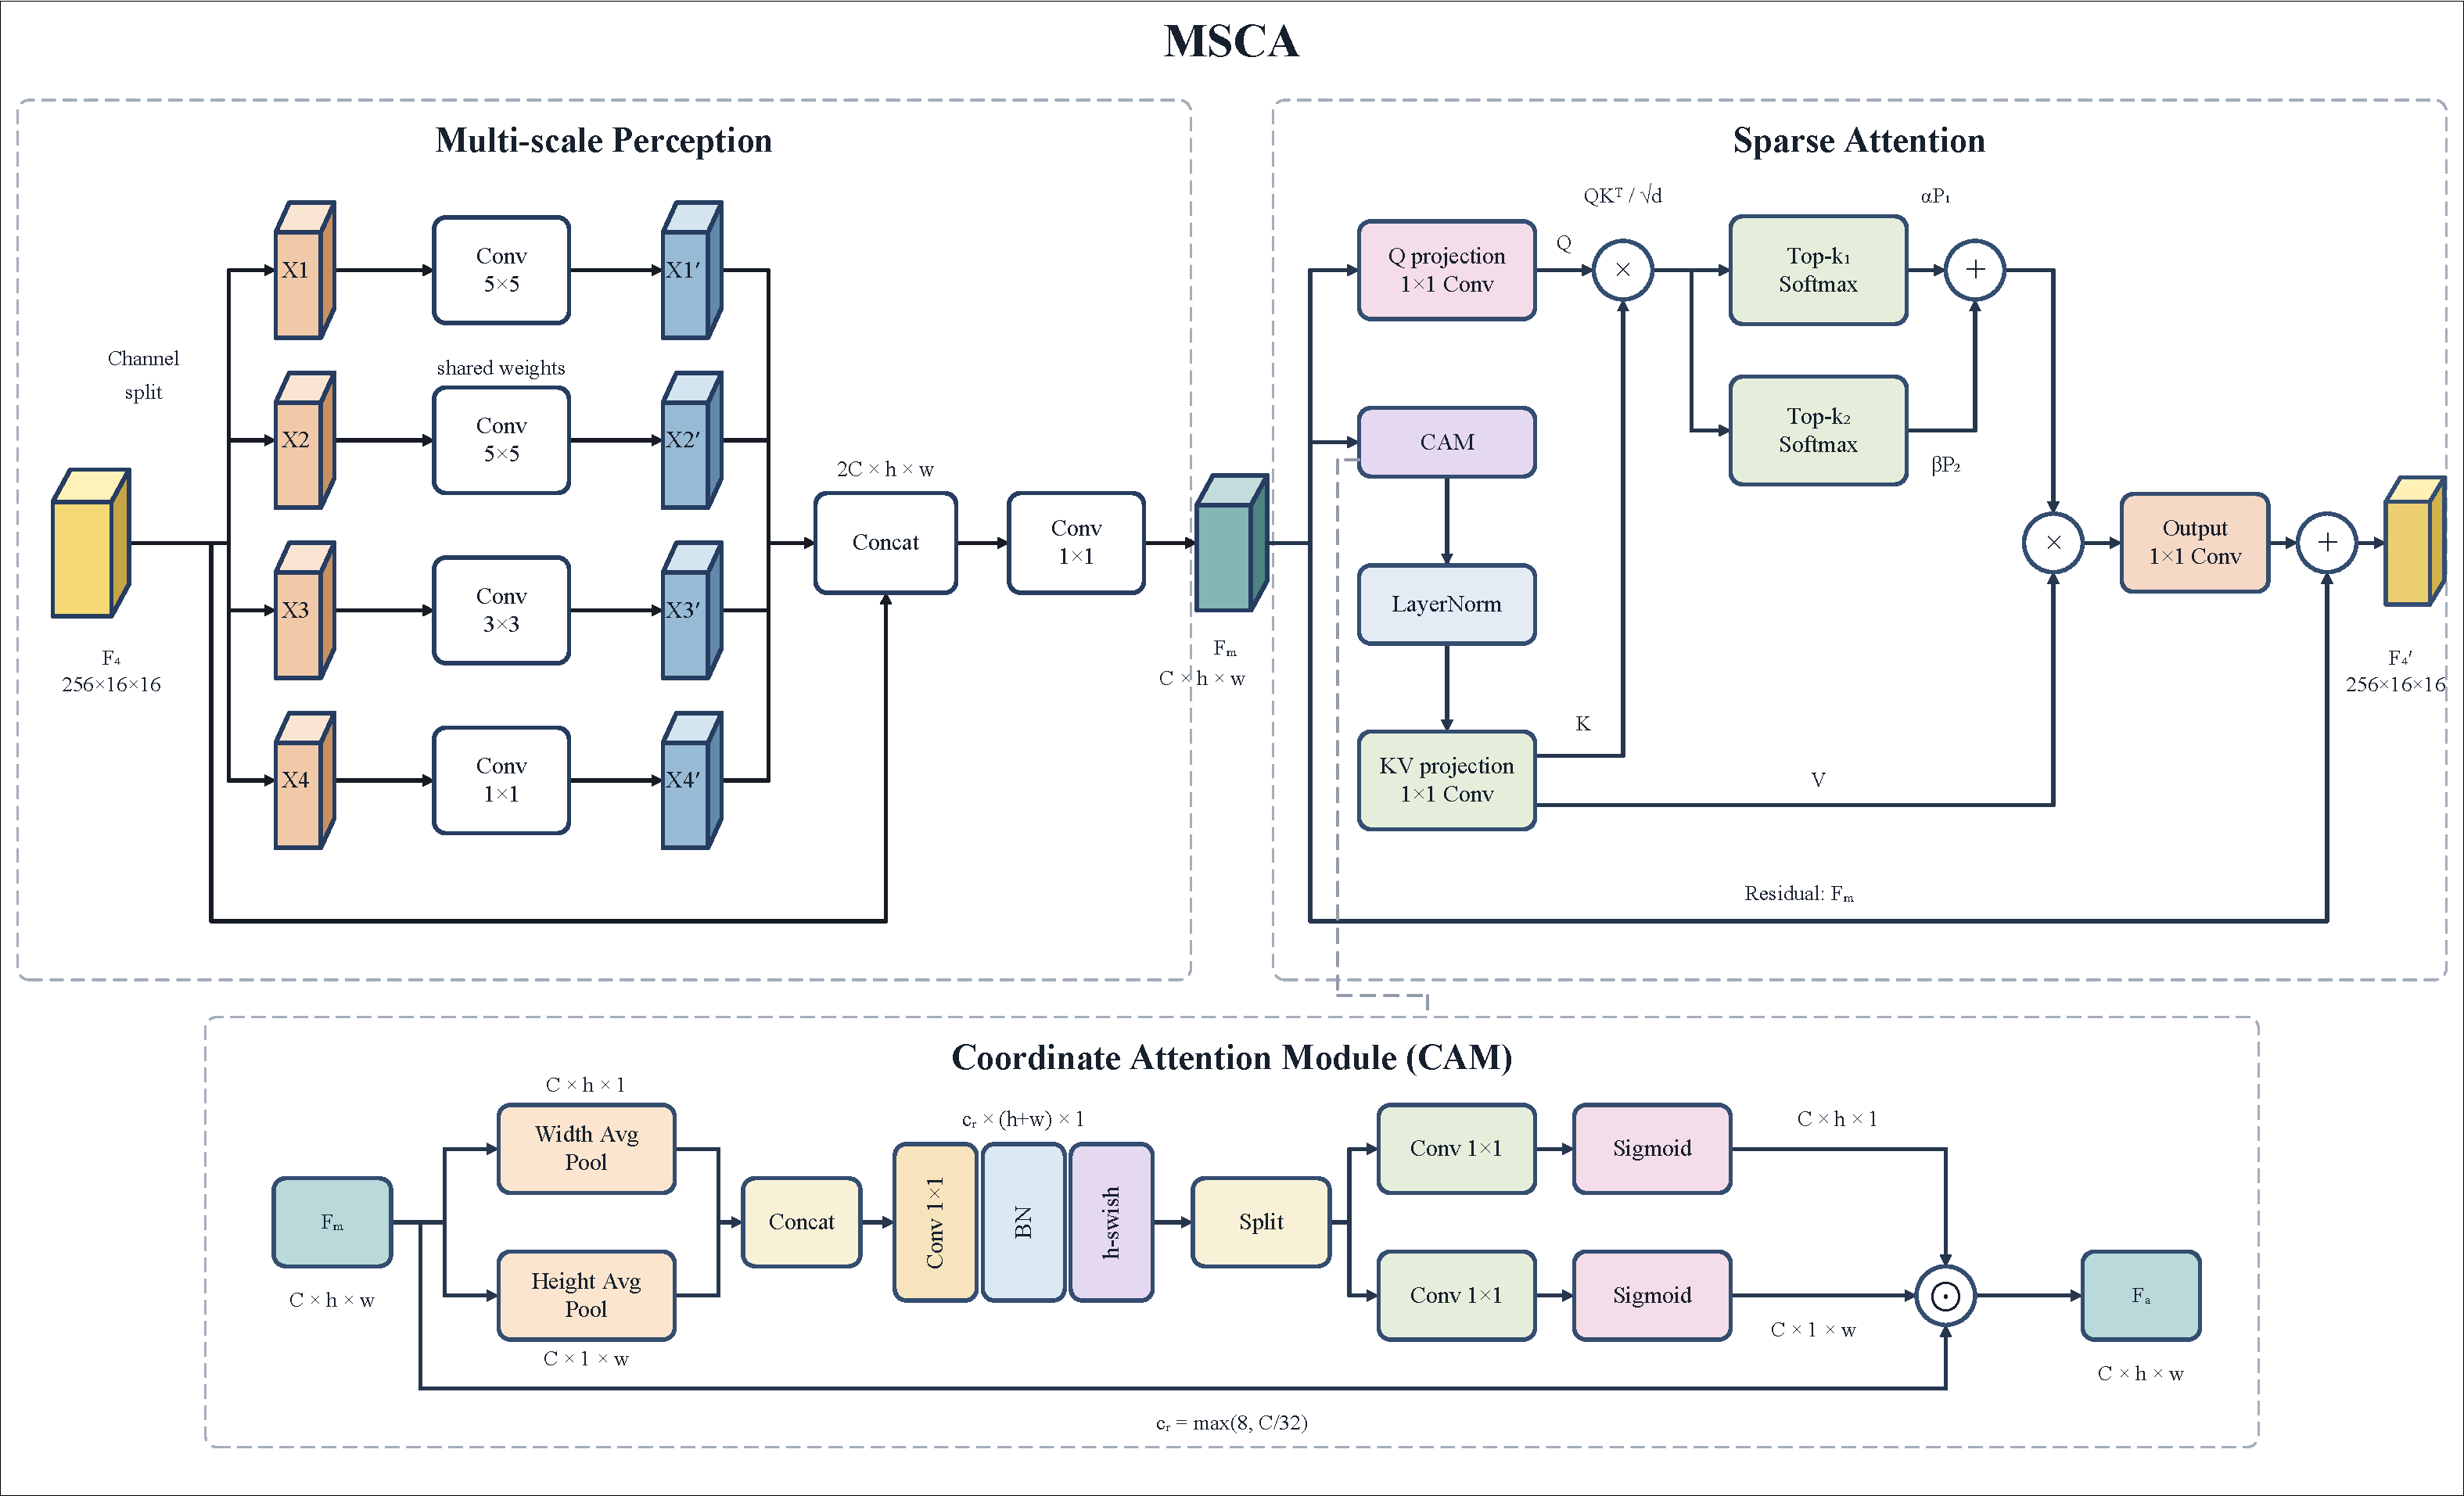
\includegraphics[width=\linewidth]{MSCA_CAM_Editable.pdf}\par
  \begin{spacing}{1}
    \methodbicaption{多尺度稀疏交叉注意力模块（MSCA）}
      {Multi-scale sparse cross-attention module (MSCA)}{fig:msca}
  \end{spacing}
  \par
\endgroup
\addvspace{6pt}

植物叶片的尺度差异与相互遮挡要求网络
同时表征局部结构和远距离空间关联。
为此，本文构建多尺度稀疏交叉注意力模块。
如图~\ref{fig:msca} 所示，
MSCA 首先提取并融合不同邻域范围的特征，
随后以融合表征生成查询，
以坐标注意力增强后的表征生成键和值，
通过双分支稀疏聚合完成空间信息交互。
该设计将多尺度感知与非对称特征交互结合，
使局部融合表征与注意力增强表征
在匹配和聚合过程中承担不同作用。

\noindent\textbf{多尺度感知}\par

在 MPCNet 的多尺度感知结构
\papercite{zhang2026mpcnet} 基础上，
将分支卷积核配置调整为 \(5\)、\(5\)、\(3\)、\(1\)，
构建用于深层特征处理的多尺度映射。
给定 \(F_4\in\mathbb{R}^{C\times h\times w}\)，
沿通道维度将其均分为四组
\(X_i\in\mathbb{R}^{(C/4)\times h\times w}\)，
分别进行卷积变换：

\begin{equation}
X_i'=\phi_{s_i}(X_i),\quad
(s_1,s_2,s_3,s_4)=(5,5,3,1)
\label{eq:msca-branches}
\end{equation}

其中，\(\phi_{s_i}\) 表示对应的卷积映射。
两个 \(5\times5\) 分支共享卷积参数，
对不同通道子集执行一致的空间变换；
\(3\times3\) 分支提取较小邻域内的结构信息，
\(1\times1\) 分支执行逐位置的通道变换。
各分支保持空间分辨率不变，
输出与原始特征沿通道维度拼接，
再通过 \(1\times1\) 卷积融合：

\begin{equation}
F_m=\phi_f\left(
\operatorname{Concat}[F_4,X_1',X_2',X_3',X_4']
\right)
\label{eq:msca-fusion}
\end{equation}

拼接特征具有 \(2C\) 个通道，
经融合映射恢复至 \(C\) 个通道，
得到 \(F_m\in\mathbb{R}^{C\times h\times w}\)。
该结构在保留原始深层表征的同时，
整合不同邻域范围内的特征响应，
为后续空间交互提供多尺度查询依据。

\noindent\textbf{坐标注意力引导的交叉注意力}\par

为在特征重标定过程中保留空间位置信息，
采用坐标注意力机制\papercite{hou2021coordinate}
构成坐标注意力模块
（Coordinate Attention Module，CAM）。
该模块分别沿宽度和高度方向进行平均池化，
经共享变换与方向分解生成两组注意力权重，
并以广播方式作用于融合特征，
得到增强表征 \(F_a\)。

以 \(F_m\) 生成查询，
以 \(F_a\) 经层归一化后的表征生成键和值：

\begin{equation}
Q=\phi_q(F_m),\quad
[K,V]=\operatorname{Split}\left(
\phi_{kv}(\operatorname{LN}(F_a))
\right)
\label{eq:msca-qkv}
\end{equation}

查询投影与键值投影均采用 \(1\times1\) 卷积，
输出通道数分别为 \(C\) 和 \(2C\)；
后者沿通道维度拆分为键和值。
层归一化在每个空间位置沿通道维度执行。
查询保留多尺度融合特征，
键和值则来自坐标注意力增强后的表征，
从而在共同的空间网格上建立
两种特征表示之间的非对称关联。

随后，对查询、键和值进行空间展平与多头重排。
设空间位置数为 \(N=hw\)，
注意力头数为 \(n_h\)，
单头通道维度为 \(d=C/n_h\)。
为简化记号，
单头特征仍记为
\(Q,K,V\in\mathbb{R}^{N\times d}\)，
其相关性矩阵为：

\begin{equation}
S=\frac{QK^{\mathsf T}}{\sqrt{d}}
\label{eq:msca-scores}
\end{equation}

矩阵 \(S\in\mathbb{R}^{N\times N}\)
描述查询位置与键位置之间的相关性，
缩放因子 \(\sqrt{d}\) 用于调节点积幅值。

\noindent\textbf{双分支稀疏聚合}\par

基于 MSCN 的双分支稀疏聚合机制
\papercite{ma2025mscn}，
对相关性矩阵采用两种保留比例进行逐行筛选，
构建不同连接密度的注意力分支：

\begin{equation}
\mathsf{P}_r=\operatorname{Softmax}\left(
\mathcal{T}_{k_r}(S)
\right),\quad r\in\{1,2\}
\label{eq:msca-sparse}
\end{equation}

权重矩阵
\(\mathsf{P}_r\in\mathbb{R}^{N\times N}\)
对应第 \(r\) 路稀疏注意力。
保留数量分别为
\(k_1=\max(1,\lfloor N/2\rfloor)\)
和 \(k_2=\max(1,\lfloor N/6\rfloor)\)。
算子 \(\mathcal{T}_{k_r}\)
保留每行最大的 \(k_r\) 个元素，
将其余元素置为负无穷；
Softmax 沿键位置维度执行，
使未保留位置的注意力权重为零。
两条分支分别提供较广泛与较集中的空间关联，
经可学习系数融合后作用于值特征：

\begin{equation}
Z=(\alpha\mathsf{P}_1+\beta\mathsf{P}_2)V
\label{eq:msca-aggregation}
\end{equation}

系数 \(\alpha\) 和 \(\beta\) 均初始化为 0.5，
用于学习两种聚合结果的贡献。
最后，拼接各注意力头的输出并恢复空间排列，
经 \(1\times1\) 卷积投影后
与融合特征残差相加：

\begin{equation}
F_4'=F_m+\phi_o\left(
\operatorname{Merge}(Z)
\right)
\label{eq:msca-output}
\end{equation}

\(\operatorname{Merge}\) 表示多头拼接与空间恢复。
输出 \(F_4'\in\mathbb{R}^{C\times h\times w}\)
保持输入尺寸，
通过残差连接整合多尺度融合表征
与稀疏聚合的空间上下文，
并作为自顶向下路径的起始特征 \(G_4\)。

\subsubsection{动态关系与上下文融合模块（DRCF）}
\begingroup
  \centering
  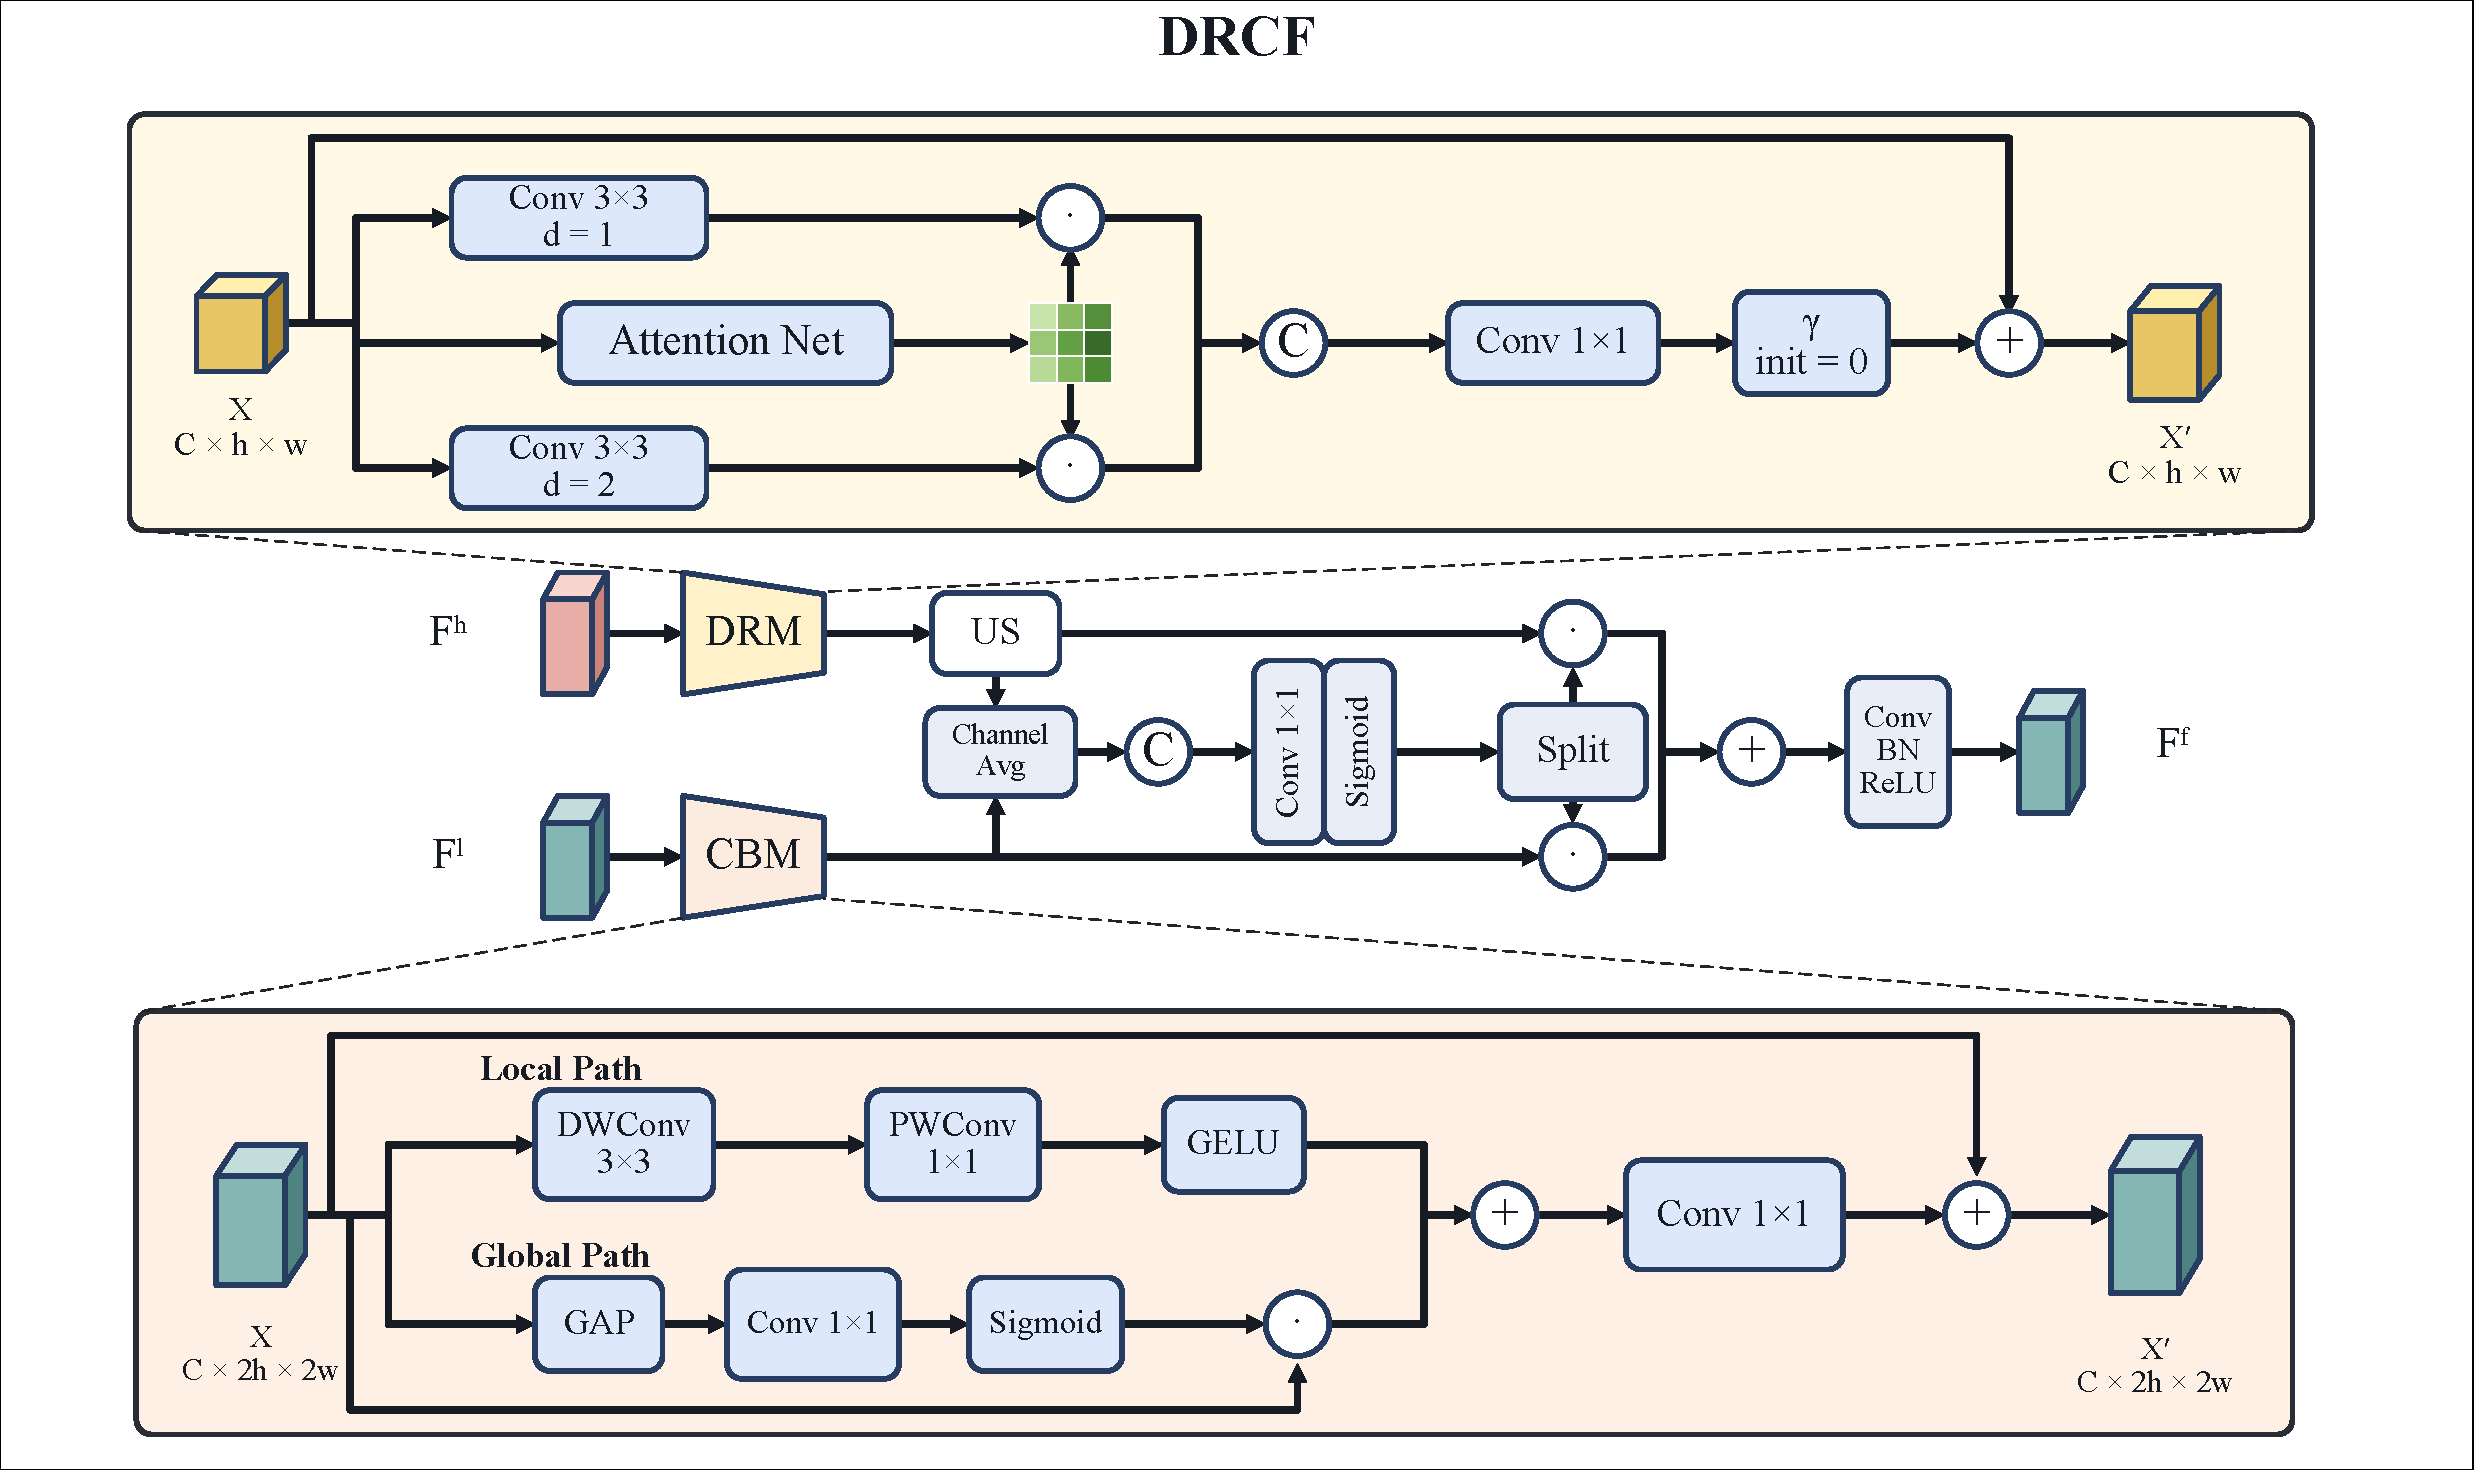
\includegraphics[width=\linewidth]{DRCF_MODA_Style.pdf}\par
  \begin{spacing}{1}
    \methodbicaption{动态关系与上下文融合模块（DRCF）}
      {Dynamic relation and context fusion module (DRCF)}{fig:drcf}
    \par\smallskip
    {\zihao{5}\normalfont
     注：上、下展开部分分别为 DRM 和 CBM；绿色方格表示
     DRM 的分支权重，对应两个经 Softmax 归一化的样本级标量。\par 
     Note: The upper and lower insets show DRM and CBM, respectively.
     The green squares represent the DRM branch weights, which are two
     sample-specific scalars normalized by softmax.\par}
  \end{spacing}
  \par
\endgroup
\addvspace{6pt}

不同层级特征在空间分辨率与语义表征上存在差异：
深层特征具有较强的语义信息，
浅层特征保留更多局部纹理与边界细节。
为实现两类信息的自适应整合，
本文构建动态关系与上下文融合模块。
采用 HyperSeg-DG 中的动态关系模块
（Dynamic Relation Module，DRM）
与上下文桥接模块
（Context Bridge Module，CBM）
\papercite{islam2026hypersegdg}
分别处理深、浅层输入，
并根据两路增强特征的空间响应
生成跨尺度融合权重。

如图~\ref{fig:drcf} 所示，
DRCF 将深层动态关系建模、
浅层上下文增强及空间自适应融合结合，
在不同分辨率之间传递语义与结构信息。
三级 DRCF 依次融合
\(G_4\) 与 \(F_3\)、\(G_3\) 与 \(F_2\)、
\(G_2\) 与 \(F_1\)，
生成 \(G_3\)、\(G_2\) 和 \(G_1\)。

\noindent\textbf{深层特征的动态关系建模}\par

给定深层输入
\(F_h\in\mathbb{R}^{C\times h\times w}\)，
采用两路膨胀率分别为 1 和 2 的
\(3\times3\) 卷积，
提取不同感受野下的特征：

\begin{equation}
D_r=\phi_{3\times3}^{(r)}(F_h),\quad r\in\{1,2\}
\label{eq:drcf-dilated}
\end{equation}

为根据输入内容调整两路响应，
利用全局平均池化提取通道描述，
经两层 \(1\times1\) 卷积与 ReLU 激活
生成分支得分，
再通过 Softmax 得到权重：

\begin{equation}
[a_1,a_2]=\operatorname{Softmax}\left(
\psi_2\left(
\operatorname{ReLU}\left(
\psi_1(\operatorname{GAP}(F_h))
\right)\right)\right)
\label{eq:drcf-branch-weights}
\end{equation}

权重 \(a_1\) 和 \(a_2\)
为随输入变化的样本级标量，
满足 \(a_1+a_2=1\)，
在通道与空间维度广播后
分别作用于两路特征。
加权结果经拼接与 \(1\times1\) 卷积融合，
再通过可学习残差系数与原始输入结合：

\begin{equation}
H=F_h+\gamma\,\phi_d\left(
\operatorname{Concat}[a_1D_1,a_2D_2]
\right)
\label{eq:drcf-drm-output}
\end{equation}

系数 \(\gamma\) 初始化为零，
使 DRM 在初始化时保持恒等映射，
并在训练过程中学习
多感受野特征对输出的贡献。

\noindent\textbf{浅层特征的上下文增强}\par

对于浅层输入
\(F_l\in\mathbb{R}^{C\times2h\times2w}\)，
CBM 通过并行的局部路径与全局路径
提取互补信息。
局部路径采用深度卷积与逐点卷积
建模邻域结构，
全局路径通过全局平均池化与 Sigmoid
生成通道门控：

\begin{equation}
L_{\mathrm{loc}}=\operatorname{GELU}\left(
\phi_{\mathrm{pw}}(\phi_{\mathrm{dw}}(F_l))
\right),\quad
g=\sigma\left(
\phi_g(\operatorname{GAP}(F_l))
\right)
\label{eq:drcf-local-global}
\end{equation}

其中，
\(\phi_{\mathrm{dw}}\) 为 \(3\times3\) 深度卷积，
\(\phi_{\mathrm{pw}}\) 为 \(1\times1\) 逐点卷积，
\(g\in\mathbb{R}^{C\times1\times1}\)
为通道门控权重。
全局路径将门控作用于原始浅层特征，
与局部路径输出相加，
经投影及残差连接得到增强特征：

\begin{equation}
L=F_l+\phi_c\left(
L_{\mathrm{loc}}+g\odot F_l
\right)
\label{eq:drcf-cbm-output}
\end{equation}

该结构在保留浅层输入的基础上，
结合局部空间变换与全局通道调节，
为跨层融合提供上下文增强的细节表征。
符号 \(\odot\) 表示逐元素乘法，
不同尺寸的权重按相应维度广播。

\noindent\textbf{空间自适应融合}\par

将深层输出双线性上采样至浅层分辨率，
得到 \(H'=\operatorname{Up}(H)\)。
随后，分别沿通道维度计算两路特征的均值，
生成单通道空间描述图：

\begin{equation}
S_h=\operatorname{Mean}_c(H'),\quad
S_l=\operatorname{Mean}_c(L)
\label{eq:drcf-spatial-descriptors}
\end{equation}

将两张描述图拼接，
通过 \(1\times1\) 卷积与 Sigmoid
预测空间融合权重：

\begin{equation}
[W_h,W_l]=\operatorname{Split}\left(
\sigma\left(
\phi_w\left(
\operatorname{Concat}[S_h,S_l]
\right)\right)\right)
\label{eq:drcf-spatial-weights}
\end{equation}

权重
\(W_h,W_l\in\mathbb{R}^{1\times2h\times2w}\)
由 Sigmoid 独立生成，
在通道维度广播，
分别调节各空间位置的深层与浅层响应。
两路加权特征相加后，
经 \(1\times1\) 卷积、
批归一化与 ReLU 激活得到模块输出：

\begin{equation}
F_{\mathrm{DRCF}}=\operatorname{ReLU}\left(
\operatorname{BN}\left(
\phi_f(W_h\odot H'+W_l\odot L)
\right)\right)
\label{eq:drcf-output}
\end{equation}

输出
\(F_{\mathrm{DRCF}}\in\mathbb{R}^{C\times2h\times2w}\)
与浅层输入保持相同尺寸。
通过对深浅层特征分别增强并自适应加权，
DRCF 逐级将深层语义传递至高分辨率表征。

\subsubsection{差异引导的跨尺度自适应调制模块（DCAM）}
\begingroup
  \centering
  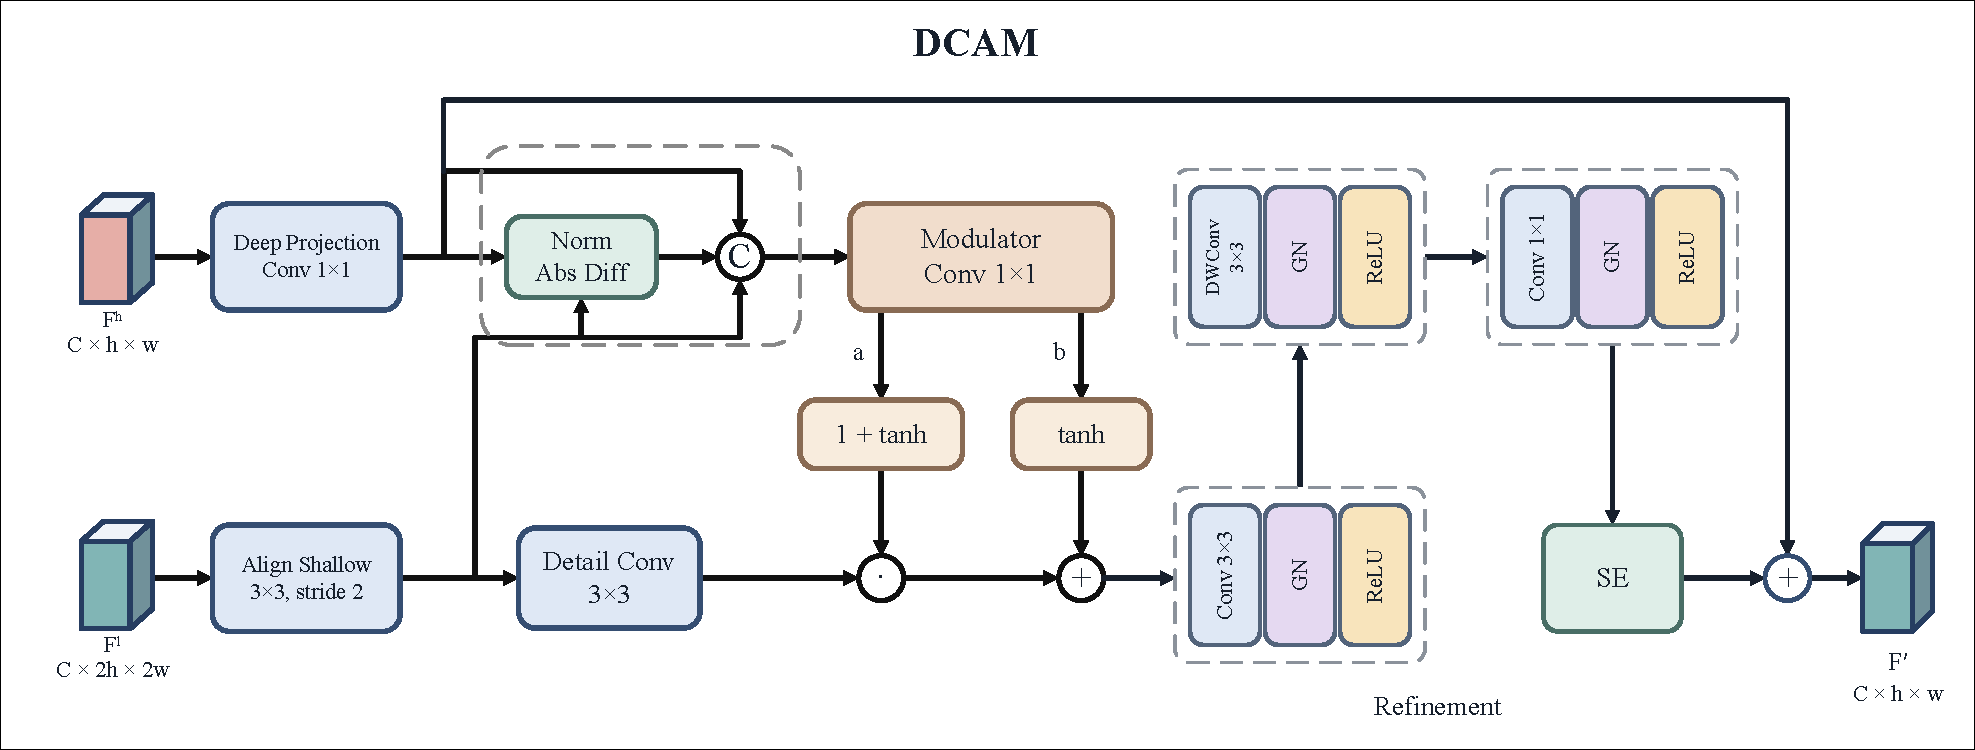
\includegraphics[width=\linewidth]{DCAM_Aligned_Editable.pdf}\par
  \begin{spacing}{1}
    \methodbicaption{差异引导的跨尺度自适应调制模块（DCAM）}
      {Difference-guided cross-scale adaptive modulation module (DCAM)}{fig:dcam}
  \end{spacing}
  \par
\endgroup
\addvspace{6pt}

跨尺度特征融合需要协调
深层语义与浅层细节之间的表征差异。
直接叠加两类特征
缺乏依据局部差异调节信息注入强度的机制。
为此，本文构建差异引导的跨尺度自适应调制模块。
如图~\ref{fig:dcam} 所示，
模块利用对齐特征及其归一化差异
生成通道与空间相关的调制参数，
对浅层细节进行乘性缩放与加性偏移，
再通过残差细化完成跨尺度信息整合。

\noindent\textbf{跨尺度特征对齐}\par

给定深层特征
\(F_h\in\mathbb{R}^{C\times h\times w}\)
和浅层特征
\(F_l\in\mathbb{R}^{C\times2h\times2w}\)，
分别通过深层投影与浅层对齐得到：

\begin{equation}
T=\phi_p(F_h),\quad S=\phi_a(F_l)
\label{eq:dcam-alignment}
\end{equation}

深层投影 \(\phi_p\)
采用 \(1\times1\) 卷积进行通道映射；
浅层对齐 \(\phi_a\)
采用步长为 2 的 \(3\times3\) 卷积，
结合组归一化与 ReLU 激活完成下采样。
两路输出均为 \(C\times h\times w\)，
为逐位置差异计算与特征调制
建立统一的空间和通道维度。

\noindent\textbf{差异引导的调制参数生成}\par

为减弱特征幅值差异对比较结果的影响，
在每个空间位置沿通道维度进行 \(L_2\) 归一化，
再计算两路特征的逐元素绝对差异：

\begin{equation}
D=\left|\mathcal{N}(S)-\mathcal{N}(T)\right|
\label{eq:dcam-discrepancy}
\end{equation}

归一化算子定义为
\(\mathcal{N}(U)_{:,i,j}
=U_{:,i,j}/\max(\lVert U_{:,i,j}\rVert_2,\epsilon)\)，
其中 \(U_{:,i,j}\)
表示位置 \((i,j)\) 处的通道向量，
\(\epsilon\) 为数值稳定常数。
差异特征
\(D\in\mathbb{R}^{C\times h\times w}\)
描述两路表征在归一化通道响应上的差异。
将其与对齐特征拼接，
通过 \(1\times1\) 卷积生成调制参数：

\begin{equation}
[a,b]=\operatorname{Split}\left(
\phi_m\left(
\operatorname{Concat}[S,T,D]
\right)\right)
\label{eq:dcam-modulation-parameters}
\end{equation}

拼接特征具有 \(3C\) 个通道，
经调制映射 \(\phi_m\) 转换为 \(2C\) 个通道，
再拆分为
\(a,b\in\mathbb{R}^{C\times h\times w}\)。
两组参数由深浅层特征及其差异共同生成，
用于调节各通道、各空间位置的细节响应，
使浅层信息的注入强度随输入内容变化。

\noindent\textbf{细节调制与残差细化}\par

对浅层对齐特征进行 \(3\times3\) 卷积、
组归一化与 ReLU 激活，
得到细节特征 \(E=\phi_e(S)\)。
利用调制参数分别执行乘性缩放与加性偏移：

\begin{equation}
E'=E\odot\left(1+\tanh(a)\right)+\tanh(b)
\label{eq:dcam-modulation}
\end{equation}

乘性系数 \(1+\tanh(a)\)
的取值范围为 \((0,2)\)，
用于调节细节响应强度；
偏移项 \(\tanh(b)\)
的取值范围为 \((-1,1)\)，
提供加性调整。
调制卷积 \(\phi_m\) 的权重与偏置均初始化为零，
使初始调制满足 \(E'=E\)，
训练过程中再学习偏离恒等调制的幅度。

调制结果依次经过 \(3\times3\) 卷积、
\(3\times3\) 深度卷积和 \(1\times1\) 逐点卷积，
各卷积后均接组归一化与 ReLU 激活。
随后，采用挤压与激励单元
（Squeeze-and-Excitation，SE）
\papercite{hu2018senet}
进行通道重标定，得到细化特征：

\begin{equation}
R=\operatorname{SE}\left(
\rho_{\mathrm{pw}}\left(
\rho_{\mathrm{dw}}\left(
\rho_{3\times3}(E')
\right)\right)\right)
\label{eq:dcam-refinement}
\end{equation}

其中，
\(\rho_{3\times3}\)、\(\rho_{\mathrm{dw}}\)
和 \(\rho_{\mathrm{pw}}\)
分别表示上述三类卷积及其归一化、激活操作。
最终将细化结果与深层投影特征残差相加：

\begin{equation}
F'=T+R
\label{eq:dcam-output}
\end{equation}

模块输出与深层输入保持相同尺寸，
以深层投影特征为残差基础，
整合经过差异引导调制与细化的浅层信息。
在自底向上路径中，
三级 DCAM 分别以
\(G_2\)、\(G_3\) 和 \(G_4\) 为深层输入，
以 \(P_1\)、\(P_2\) 和 \(P_3\) 为浅层输入，
依次生成 \(P_2\)、\(P_3\) 和 \(P_4\)，
完成浅层细节向深层表征的逐级反馈。

\subsubsection{分割输出与损失函数}

\noindent\textbf{前景辅助监督与残差增强}\par

在自顶向下路径的最浅层融合特征 \(G_1\)
上设置辅助预测头，
生成单通道前景响应 \(A\)，
经 Sigmoid 得到前景概率图 \(M\)。
利用前景概率对融合特征进行残差加权，
再通过通道映射形成
自底向上路径的起始特征：

\begin{equation}
A=\phi_{\mathrm{aux}}(G_1),\quad
M=\sigma(A),\quad
P_1=\phi_s\left(G_1\odot(1+M)\right)
\label{eq:prediction-foreground}
\end{equation}

辅助预测头由 \(3\times3\) 卷积、
组归一化、ReLU 和 \(1\times1\) 输出卷积组成。
概率图 \(M\) 在通道维度广播，
使残差加权在保留原始特征分量的基础上
增强前景响应。
随后，三级 DCAM 逐级融合浅层细节与深层语义，
生成 \(P_2\)、\(P_3\) 和 \(P_4\)。

\noindent\textbf{多尺度解码与细节融合}\par

将 \(P_1\) 至 \(P_4\)
对齐至输入图像的四分之一分辨率，
沿通道维度拼接后，
通过卷积解码器得到融合特征 \(U\)。
同时，将输入图像缩放至二分之一分辨率，
通过 RGB 细节分支提取局部特征
\(E_{\mathrm{rgb}}\)。
解码特征上采样后与细节特征拼接，
经分割预测头生成类别响应，
并恢复至输入尺寸：

\begin{equation}
O=\mathcal{U}_1\left(
\phi_{\mathrm{seg}}\left(
\operatorname{Concat}[
\mathcal{U}_{1/2}(U),E_{\mathrm{rgb}}
]\right)\right)
\label{eq:prediction-output}
\end{equation}

其中，
\(\mathcal{U}_{1/2}\) 和 \(\mathcal{U}_1\)
分别表示对齐至输入图像二分之一分辨率
和原始分辨率的双线性插值。
解码器通过两个 \(3\times3\) 卷积块，
将拼接特征的通道数依次压缩至 256 和 64；
RGB 分支通过两个 \(3\times3\) 卷积块
生成 32 通道细节特征。
分割预测头由 \(3\times3\) 卷积块
和 \(1\times1\) 分类卷积组成。
本节中的卷积块均由卷积、
组归一化与 ReLU 激活组成。
最终输出为
\(O\in\mathbb{R}^{K\times H\times W}\)，
其中 \(K\) 为包含背景的类别总数。
推理时，选取各像素最大类别响应
对应的类别作为分割结果。

\noindent\textbf{联合训练目标}\par

主分割分支采用像素级交叉熵损失
与前景 Dice 损失联合监督。
交叉熵约束像素类别预测，
Dice 损失约束预测区域与真实区域的重叠，
对每幅图像的各前景类别分别计算后，
在样本与类别维度取平均：

\begin{equation}
\mathcal{L}_{\mathrm{Dice}}
=1-\frac{1}{B(K-1)}
\sum_{b=1}^{B}\sum_{c=1}^{K-1}
\frac{2\sum_i p_{bic}y_{bic}+\epsilon_d}
{\sum_i p_{bic}+\sum_i y_{bic}+\epsilon_d}
\label{eq:loss-dice}
\end{equation}

其中，\(B\) 为批量大小，
\(i\) 遍历图像中的像素，
\(c\) 表示类别；
\(p_{bic}\) 为对输出 \(O\)
沿类别维度执行 Softmax 后得到的预测概率，
\(y_{bic}\) 为对应的独热标签。
背景类别编号为 0，不参与 Dice 平均，
平滑项设置为 \(\epsilon_d=1\)。

辅助分支将所有非背景类别合并为前景，
采用二元交叉熵监督
上采样至标签分辨率的辅助响应 \(A\)。
训练时直接根据辅助响应计算带 logits 的二元交叉熵，
以提高数值稳定性。
最终训练目标为：

\begin{equation}
\mathcal{L}
=\mathcal{L}_{\mathrm{CE}}
+\lambda_d\mathcal{L}_{\mathrm{Dice}}
+\lambda_a\mathcal{L}_{\mathrm{aux}}
\label{eq:loss-total}
\end{equation}

设置 \(\lambda_d=1\)、\(\lambda_a=0.2\)。
主分割监督共同约束像素类别与前景区域重叠，
辅助监督为前景增强分支提供直接的区域约束，
三者联合优化网络参数。
\par
\endgroup